% ============================================================
%  CHAPITRE 2 — Section 4 : EMS considérées
% ============================================================

\section{EMS considérées}
\label{sec:ems}

Cette section présente les différentes EMS qui ont été conçues et simulées dans le cadre d'évaluation décrit précédemment. L'objectif est d'explorer un éventail de philosophies de contrôle suffisamment large pour couvrir les principaux compromis réalisables dans le plan de Pareto, et d'identifier parmi elles la stratégie offrant le meilleur équilibre entre fiabilité d'alimentation et préservation des composants. Toutes les EMS présentées ici sont des stratégies en ligne, c'est-à-dire qu'elles ne s'appuient pas sur la connaissance du futur et sont compatibles avec une implémentation temps réel dans le microréseau.

% ------------------------------------------------------------
\subsection{Power-splitting \& frequency splitting}
% ------------------------------------------------------------

La première famille de stratégies repose sur une répartition statique de la puissance entre la batterie et le sous-système hydrogène. Ces configurations sont caractérisées par des ratios de distribution fixes de la puissance de référence totale $\hat{P}_{\text{tot,plan}} = (\hat{P}_{\text{Load}} - \hat{P}_{\text{PV}})$ entre les deux médias de stockage~:
\[
(100-0), \quad (75-25), \quad (50-50), \quad (25-75), \quad (0-100)
\]
où le premier terme correspond à la part [\%] attribuée à la batterie et le second au système hydrogène. Ces stratégies vont donc d'une philosophie attribuant l'essentiel du travail à la batterie à une philosophie le confiant principalement aux composants hydrogène~\cite{eldeeb_hybrid_2019}.

Cette approche est structurellement proche des stratégies de \textit{frequency splitting}, dans lesquelles deux composants de stockage aux dynamiques temporelles différentes se partagent différentes bandes du spectre fréquentiel de la charge~\cite{corapsiz_overview_2023}. Dans ce type de stratégie, la batterie, plus rapide, absorbe les fluctuations hautes fréquences, tandis que le système hydrogène, plus lent, gère les composantes basses fréquences. Le \textit{power splitting} a toutefois été préféré ici au \textit{frequency splitting}, car il conduit à de meilleurs résultats sur les indicateurs retenus pour ce cas d'étude particulier.

% ------------------------------------------------------------
\subsection{SoC-based}
% ------------------------------------------------------------

Deux lois de contrôle supplémentaires ont été implémentées pour maintenir le SoC de la batterie autour de cibles spécifiques. La première vise à maintenir $\text{SoC}_{\text{bat}}$ proche de $0{,}6$ (notée SoC06), ce qui représente un état équilibré permettant à la fois des marges de charge et de décharge. La seconde cherche à maintenir $\text{SoC}_{\text{bat}}$ proche de $1$ (SoC1), favorisant la disponibilité de l'énergie stockée pour les consommateurs, mais pouvant accroître la dégradation en raison d'un fonctionnement prolongé à SoC élevé. Ces philosophies de contrôle sont également des approches très répandues dans les systèmes électriques hybrides~\cite{sorrentino_real-time_2021}\cite{zou_real-time_2023}.

Dans ces deux stratégies, le sous-système hydrogène joue un rôle d'appui à la batterie~: la pile à combustible est sollicitée pour recharger la batterie lorsque son SoC descend en dessous de la cible, et l'électrolyseur absorbe l'excès de production PV lorsque la batterie est pleine. Cette dépendance forte vis-à-vis des composants hydrogène a des conséquences directes sur leur niveau de sollicitation et donc sur leur dégradation, comme le montreront les résultats.

% ------------------------------------------------------------
\subsection{Autres stratégies}
% ------------------------------------------------------------

Des stratégies à base de règles plus élaborées ont également été implémentées afin de concilier réactivité dynamique et simplicité de calcul. Ces deux stratégies, notées RB1 et RB2, sont décrites ci-après et illustrées à la Figure~\ref{fig:RB_ems}.

\paragraph{Stratégie RB1.}
La stratégie RB1 définit le partage de puissance en fonction du SoC de la batterie au travers de règles par morceaux. Lorsque le SoC se trouve dans la plage intermédiaire ($0{,}2 < \text{SoC}_{\text{bat}} < 0{,}6$), la puissance de référence totale $\hat{P}_{\text{tot,plan}}$ est répartie linéairement entre la batterie et les composants hydrogène~: la batterie fournit la totalité de la puissance de référence lorsque le SoC atteint $0{,}6$, et aucune puissance lorsqu'il atteint $0{,}2$. En dehors de cette plage, la batterie fonctionne seule lorsque $\text{SoC}_{\text{bat}} > 0{,}6$ en décharge ou lorsque $\text{SoC}_{\text{bat}} < 0{,}2$ en charge, tandis que la pile à combustible ou l'électrolyseur prend le relais selon le sens du bilan de puissance. Cette règle assure ainsi des transitions douces entre les différents modes de fonctionnement tout en évitant les valeurs extrêmes de SoC.

\paragraph{Stratégie RB2.}
La stratégie RB2 simplifie la logique de contrôle en définissant deux modes de fonctionnement principaux. Lorsque la puissance de référence totale $\hat{P}_{\text{tot,plan}}$ est positive (la demande de charge excède la production), une puissance d'offset fixe $P_{\text{FC-offset}}$ est allouée à la pile à combustible, et la batterie fournit le complément. De façon symétrique, lorsque $\hat{P}_{\text{tot,plan}}$ est négative (excès de production), l'électrolyseur absorbe une puissance d'offset fixe $P_{\text{ELY-offset}}$, tandis que la batterie assure le reste. Ces paramètres d'offset sont ajustés par recherche des meilleures valeurs d'indicateurs. Cette logique permet aux composants hydrogène de fonctionner à des puissances plus constantes, limitant ainsi les transitoires et les cycles de démarrage-arrêt, et par conséquent prolongeant leur durée de vie.

\begin{figure}[h!]
    \centering
    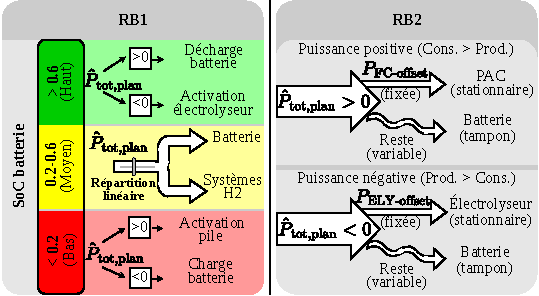
\includegraphics[width=0.8\linewidth]{Chapitre 2/EMS/Figures/RB1_2_EMS_v4.pdf}
    \caption{Illustration des stratégies RB1 et RB2.}
    \label{fig:RB_ems}
\end{figure}
\FloatBarrier

L'ensemble des neuf EMS considérées est récapitulé dans le Tableau~\ref{tab:EMS}.

\begin{table}[h!]
    \centering
    \caption{Récapitulatif des EMS implémentées.}
    \label{tab:EMS}
    \setlength{\tabcolsep}{3pt}
    \begin{tabularx}{\columnwidth}{llX}
        \hline
        Type d'EMS & Notation & Remarques \\
        \hline
        Power split & (X-Y) & $X, Y \in \{0, 25, 50, 75, 100\}$ [\%], parts batterie-hydrogène. \\
        \noalign{\smallskip}
        SoC cible & SoCX & $X \in \{0{,}6\,;\,1\}$~: SoC cible pour la batterie. \\
        \noalign{\smallskip}
        Règles élaborées & RBX & $X \in \{1, 2\}$~: logique décrite à la Fig.~\ref{fig:RB_ems}. \\
        \hline
    \end{tabularx}
\end{table}

% ------------------------------------------------------------
\subsection{Paramètres de simulation \& hypothèses}
% ------------------------------------------------------------

Les paramètres principaux de simulation ainsi que les hypothèses retenues sont rappelés ici pour mémoire, l'algorithme de simulation ayant été décrit à la section précédente. Le système modélisé est le microréseau hybride DC isolé de La Réunion, dont l'architecture et le dimensionnement ont été présentés au chapitre précédent. Les principales données de dimensionnement sont rappelées dans le Tableau~\ref{tab:system_parameters} pour faciliter la lecture des résultats.

\begin{table}[h!]
    \centering
    \caption{Principaux paramètres et dimensionnement du microréseau hybride.}
    \label{tab:system_parameters}
    \begin{tabular}{lcr}
        \hline
        Description & Symbole & Valeur nominale \\
        \hline
        Puissance de charge moyenne         & $\overline{P}_{\text{Load}}$  & 2,2 kW  \\
        Puissance de charge maximale        & $P_{\text{Load,max}}$         & 4,2 kW  \\
        Puissance PV maximale               & $P_{\text{PV,max}}$           & 32,7 kW \\
        Capacité nominale de la batterie    & $E_{\text{bat,nom}}$          & 39 kWh  \\
        Puissance nominale PEMFC            & $P_{\text{FC,max}}$           & 1,5 kW  \\
        Puissance nominale PEMWE            & $P_{\text{ELY,max}}$          & 16 kW   \\
        Capacité de stockage hydrogène      & $E_{\text{H2,max}}$           & 200 kWh \\
        \hline
    \end{tabular}
\end{table}

L'analyse est conduite à dimensionnement fixé~: les tailles des composants ne varient pas d'une simulation à l'autre, ce qui garantit que les différences observées entre EMS sont uniquement imputables aux décisions de contrôle et non à des effets de dimensionnement. Ce choix, bien qu'il ne reflète pas nécessairement une configuration physiquement ou économiquement optimisée, permet une comparaison claire et équitable des stratégies. Les profils de puissance utilisés sont issus de relevés de terrain réalisés à La Réunion, reflétant les habitudes de consommation des résidents locaux et la production solaire caractéristique du site.

Concernant les méthodes d'estimation du SoH, détaillées à la section~\ref{sec:soh}, il est supposé que les techniques existantes permettent un suivi suffisamment précis pour que les plages de fonctionnement actualisées correspondent à la réalité. Cette hypothèse, qui fonde l'approche réactive au vieillissement commune à toutes les EMS, est éprouvée à la section~\ref{sec:sensibilite} au regard d'un bruit sur l'estimation du SoH.

% ------------------------------------------------------------
\section{Résultats préliminaires}
% ------------------------------------------------------------
\subsection{LPSP et dégradation des composants }
\label{sec:resultats}
L'ensemble des neuf EMS décrites ci-dessus a été simulé sur un horizon de vingt-cinq ans, et leurs performances sont représentées dans le plan de Pareto à la Figure~\ref{fig:pareto}. Cette sous-section en présente d'abord les résultats nominaux, lorsque tous les composants sont opérationnels, avant d'en discuter les enseignements et les implications économiques.

% ------------------------------------------------------------
\subsubsection{Résultats}
\label{subsec:pareto_resultats}
% ------------------------------------------------------------

\begin{figure}[h!]
    \centering
    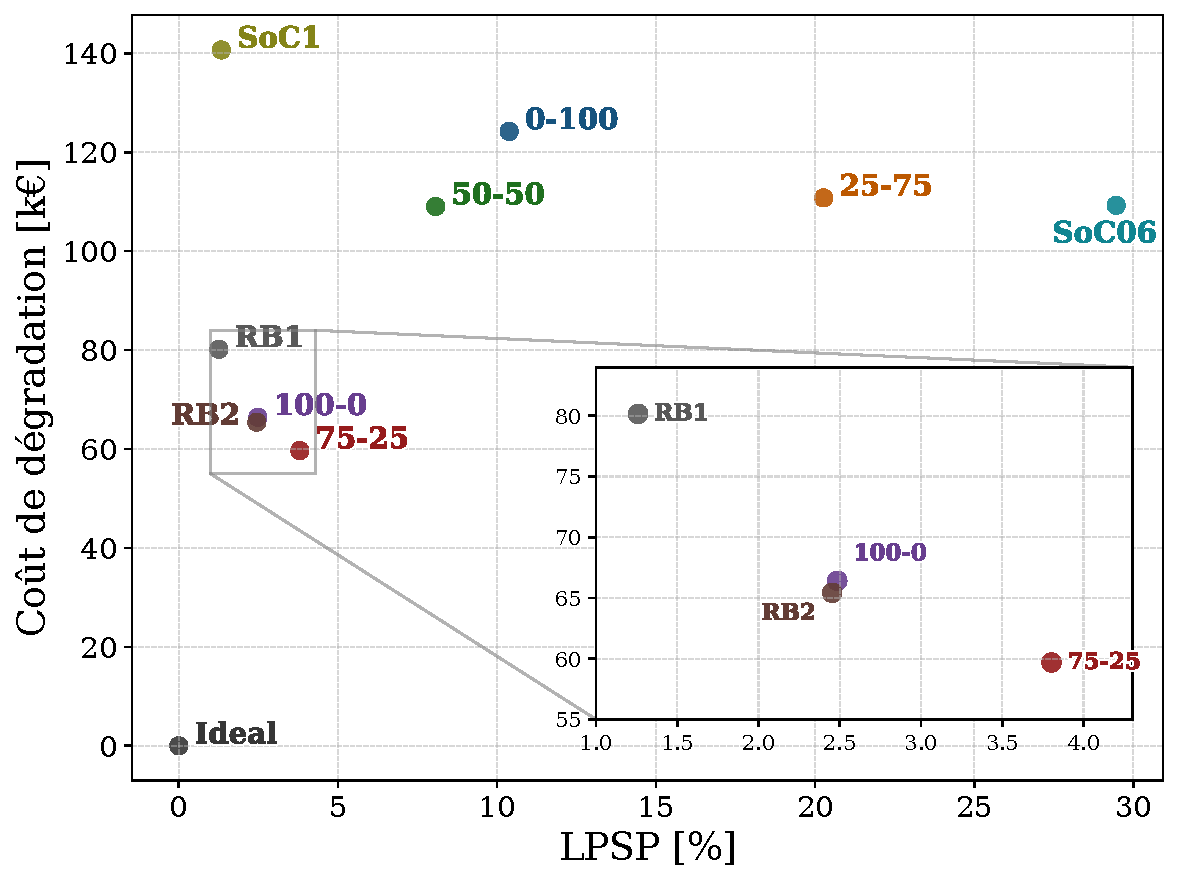
\includegraphics[width=.8\linewidth]{Chapitre 2/EMS/Figures/pareto_ems.pdf}
    \caption{Visualisation des neuf EMS dans le plan de Pareto pour une simulation de vingt-cinq ans.}
    \label{fig:pareto}
\end{figure}
\FloatBarrier

Plusieurs enseignements se dégagent de cette représentation. Les stratégies de \textit{power splitting} apparaissent déjà pertinentes, mais leurs performances sont, comme attendu, fortement dépendantes de la part de puissance assurée par la batterie. Il a été observé qu'une utilisation plus importante de la batterie conduit à une réduction significative des coûts de dégradation~: environ $-46{,}5\,\%$ en passant de l'EMS $0$-$100$ (124~k€) à l'EMS $100$-$0$ (66~k€), les composants hydrogène étant particulièrement sujets à la dégradation. Cette tendance s'accompagne également d'une nette amélioration de la qualité de service ($-76{,}1\,\%$ de LPSP, qui chute de $10{,}4\,\%$ à $2{,}5\,\%$). Ce résultat s'explique par le fait que la batterie, grâce à ses meilleures propriétés dynamiques, est plus à même de répondre rapidement aux fluctuations de charge, là où les composants hydrogène peinent à suivre des variations rapides sans s'user prématurément.

Les stratégies à SoC cible offrent des résultats plus extrêmes. Selon la valeur cible retenue, elles peuvent se révéler à la fois les meilleures et les moins bonnes stratégies en termes de LPSP, mais s'accompagnent systématiquement de coûts de dégradation élevés. La stratégie SoC1, qui maintient la batterie quasiment pleine, atteint une excellente disponibilité (LPSP $\approx 1{,}3\,\%$) mais au prix du coût de dégradation le plus élevé du panel ($\approx 141$~k€)~: garder la batterie à plein SoC impose en effet de solliciter en permanence la pile à combustible pour la recharger, et expose en outre la batterie à un vieillissement calendaire accru. À l'opposé, SoC06, qui vise un SoC médian, dégrade fortement le service (LPSP $\approx 29\,\%$) car elle écrête volontiers l'énergie disponible pour rester proche de la cible, privant les usagers d'une réserve pourtant présente. Ce comportement s'explique, dans les deux cas, par le fait que les composants hydrogène sont entièrement asservis au maintien de la cible de SoC, ce qui les soumet à une sollicitation intense et régulière, délétère pour leur durée de vie.

La stratégie RB1, qui module continûment le partage en fonction du SoC, réalise quant à elle la plus faible LPSP de toutes les stratégies ($\approx 1{,}3\,\%$) pour un coût de dégradation intermédiaire ($\approx 80$~k€). Elle illustre l'intérêt d'une transition douce entre modes de fonctionnement~; son coût reste toutefois supérieur à celui de RB2, car ses transitions progressives sollicitent davantage les composants hydrogène en régime variable que l'offset constant de RB2.

Parmi toutes les stratégies testées, la stratégie à base de règles RB2 apparaît comme offrant le compromis le plus équilibré entre continuité de service et longévité des composants. Elle atteint une LPSP d'environ $2{,}45\,\%$ pour un coût de dégradation d'environ $65{,}4$~k€, se positionnant ainsi près du front de Pareto tout en maintenant des niveaux de LPSP et de dégradation raisonnables. Elle domine notamment légèrement l'EMS $100$-$0$, dont elle reprend la philosophie « tout-batterie » mais qu'elle améliore en allouant aux composants hydrogène une puissance d'offset constante, plus douce pour leur vieillissement. Ce caractère équilibré fait de RB2 la candidate la plus prometteuse en vue d'une amélioration ultérieure.

Le fonctionnement de la stratégie RB2 sur l'horizon complet est illustré à la Figure~\ref{fig:rb2_curves}, qui présente l'évolution des puissances sur vingt-cinq ans ainsi qu'un agrandissement sur une semaine. La batterie y absorbe l'essentiel des fluctuations rapides du déséquilibre entre production et demande, tandis que la pile à combustible et l'électrolyseur fonctionnent par paliers, à une puissance d'offset sensiblement constante entrecoupée de phases d'arrêt. Le suivi du SoC de la batterie et du niveau du réservoir d'hydrogène confirme que les réserves restent dans des plages de fonctionnement saines, les pertes d'alimentation demeurant rares et de faible amplitude.

\begin{figure}[h!]
    \centering
    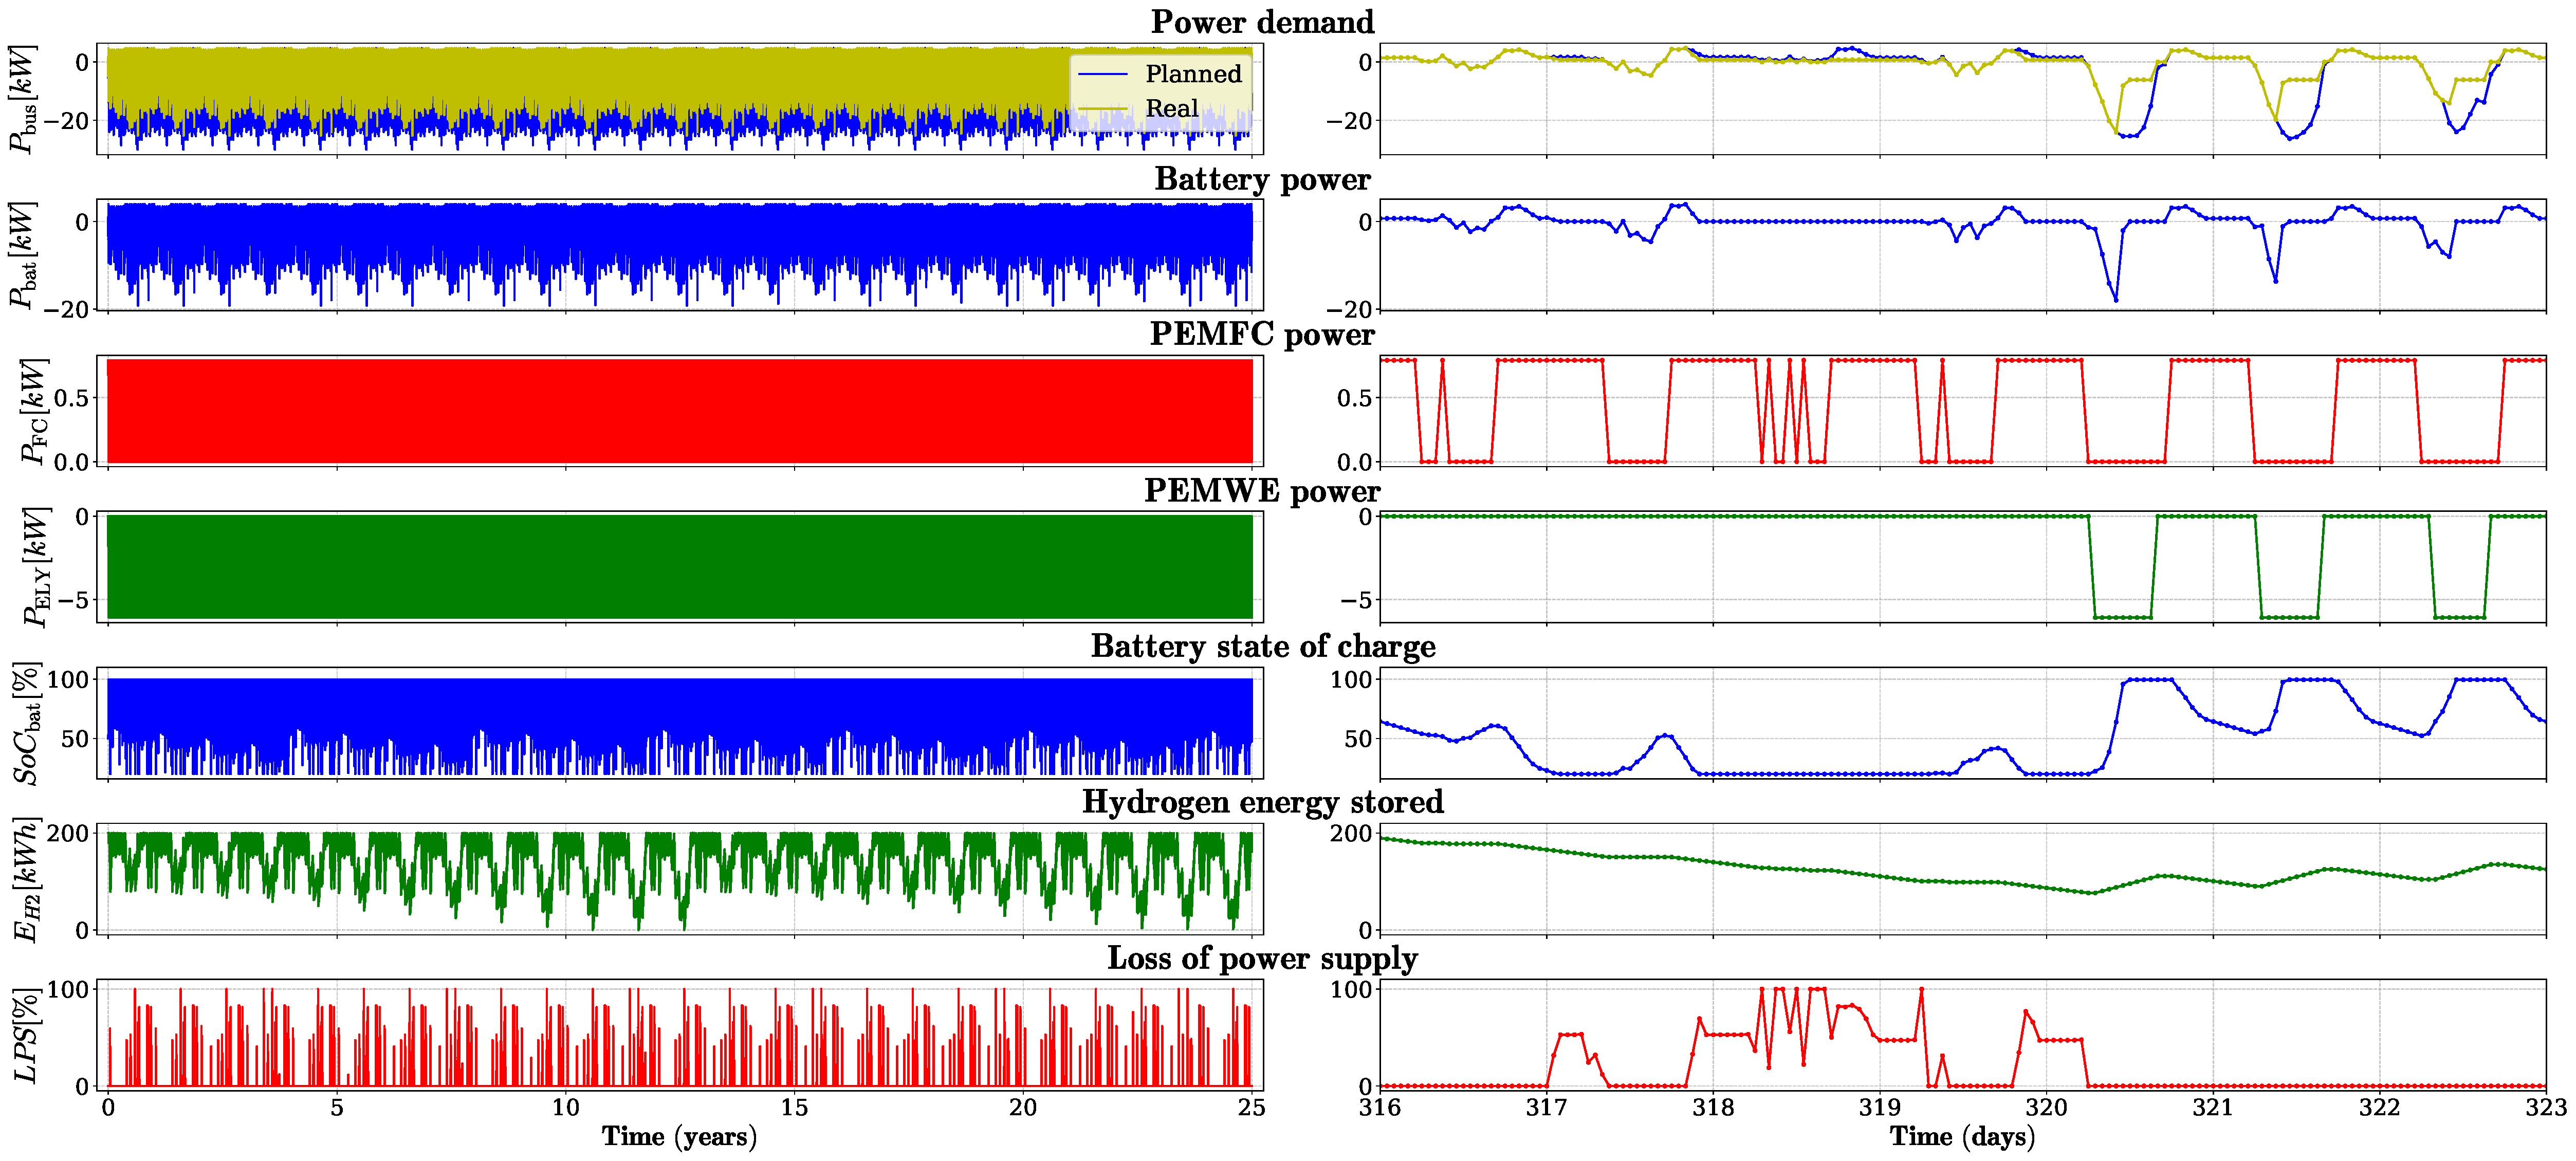
\includegraphics[width=\linewidth]{Chapitre 2/EMS/Figures/everything_combined_v2_2.pdf}
    \caption{Profils de puissance de la stratégie RB2~: simulation sur vingt-cinq ans (gauche) et agrandissement sur une semaine (droite).}
    \label{fig:rb2_curves}
\end{figure}
\FloatBarrier

L'évolution du vieillissement des composants et la décomposition de leur dégradation sont reportées à la Figure~\ref{fig:rb2_aging}. Les courbes de SoH font apparaître les remplacements périodiques évoqués plus haut, la batterie étant de loin le composant le plus fréquemment remplacé. La répartition des mécanismes de dégradation est plus instructive encore~: pour la pile à combustible, les cycles de démarrage-arrêt constituent de loin la cause dominante, avec près de $96\,\%$ de la dégradation totale~; pour l'électrolyseur, la dégradation est principalement portée par la contribution irréversible associée au fonctionnement soutenu à forte puissance (environ $59\,\%$), les démarrages-arrêts n'en représentant qu'environ $36\,\%$.

\begin{figure}[h!]
    \centering
    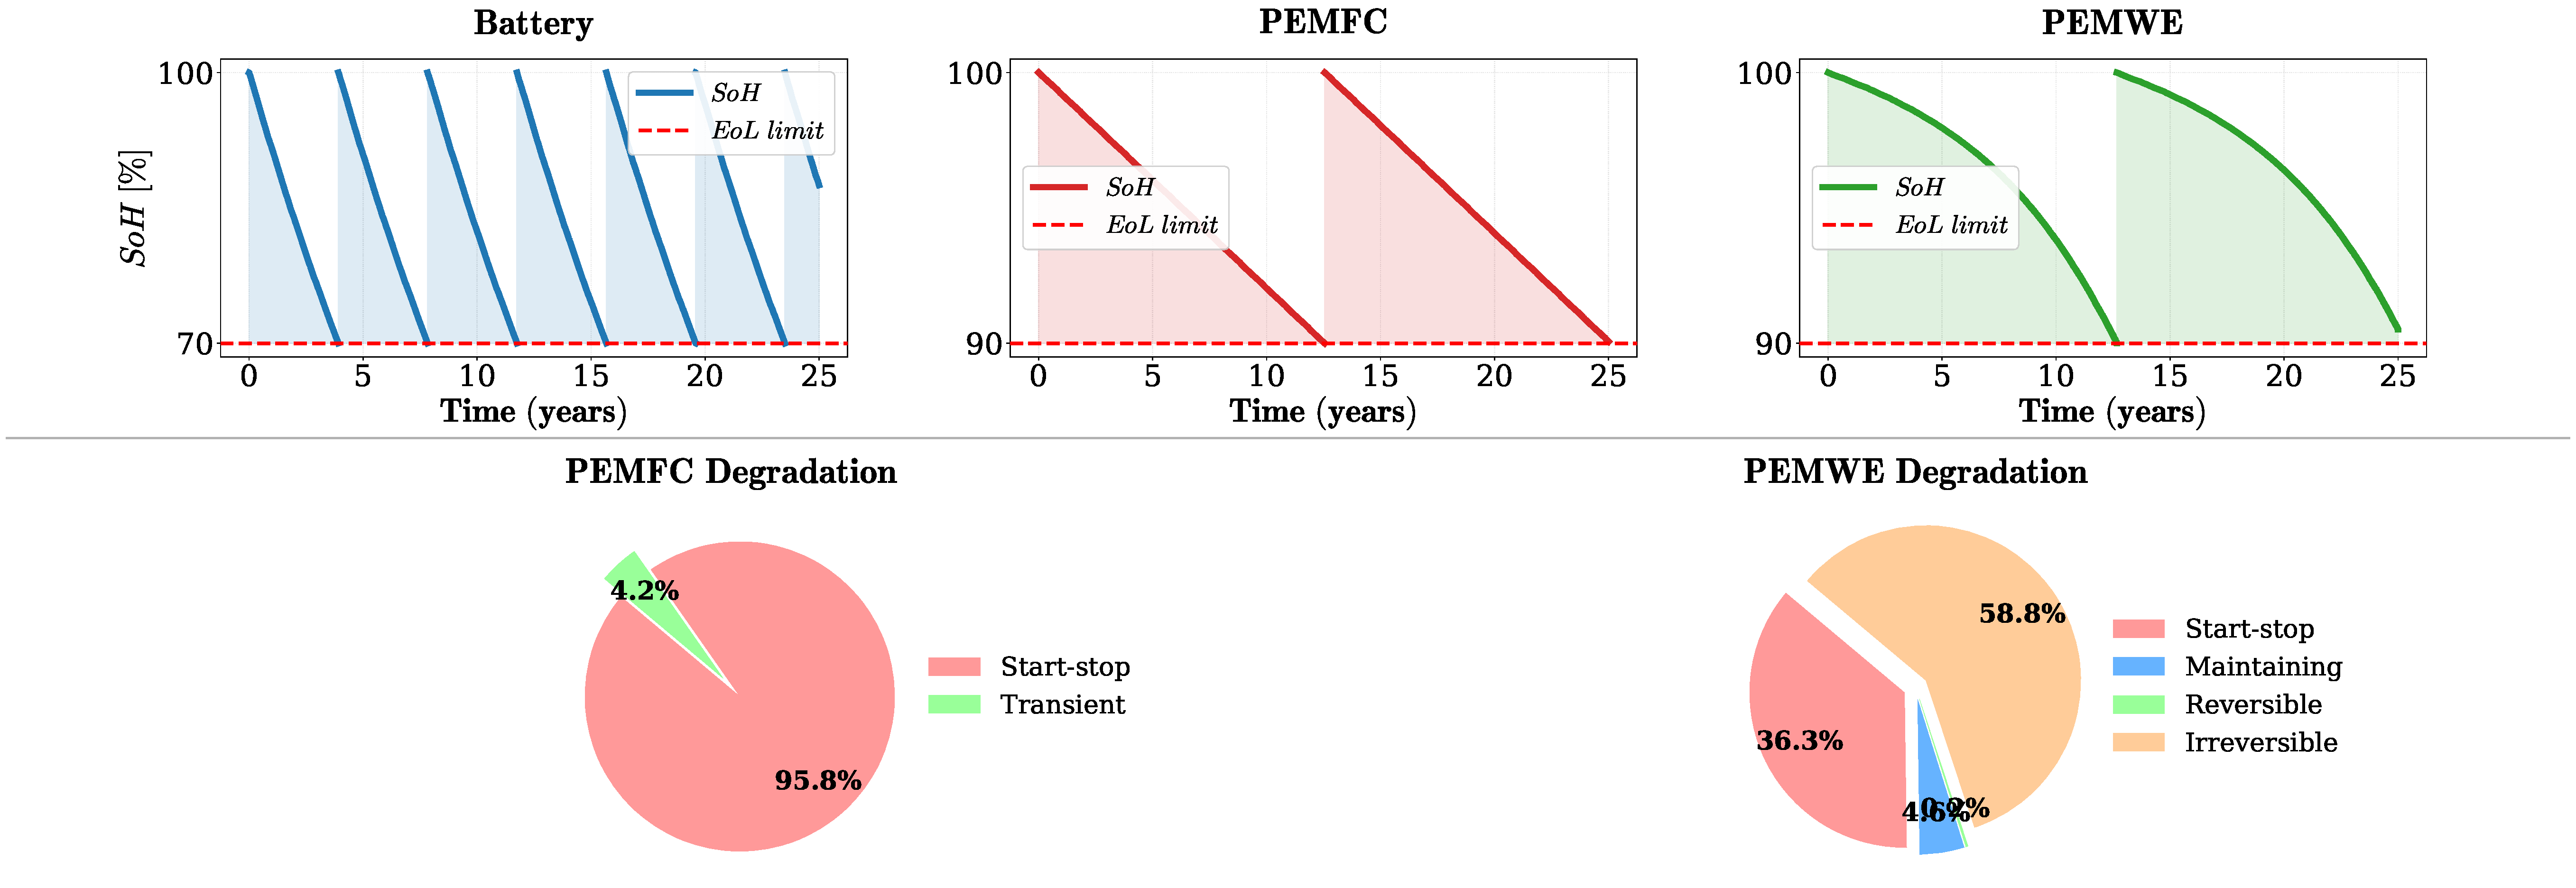
\includegraphics[width=\linewidth]{Chapitre 2/EMS/Figures/all_aging_2.pdf}
    \caption{Vieillissement sous la stratégie RB2~: évolution du SoH des composants (haut) et répartition des mécanismes de dégradation des composants hydrogène (bas).}
    \label{fig:rb2_aging}
\end{figure}
\FloatBarrier

% ------------------------------------------------------------
\subsubsection{Discussion}
% ------------------------------------------------------------

D'un point de vue économique, les coûts équivalents associés à la dégradation des composants s'échelonnent, sur vingt-cinq ans, de l'ordre de 60~k€ à près de 141~k€ selon l'EMS retenue, ce qui souligne l'importance cruciale du choix de la stratégie de contrôle pour l'opération du système. Ces coûts sont liés aux remplacements périodiques des composants, dont les fréquences sont estimées à environ une fois tous les quatre ans pour la batterie, tous les douze à treize ans pour la pile à combustible et tous les treize ans pour l'électrolyseur. Le vieillissement relativement rapide de la batterie est cohérent avec la chimie lithium-ion NMC considérée et avec son dimensionnement modeste, qui impose des cycles profonds et fréquents~; ces durées de vie absolues doivent toutefois être lues comme des estimations dépendantes du modèle et du dimensionnement plutôt que comme des valeurs validées expérimentalement~\cite{madani_comprehensive_2025}\cite{superchi_importance_2025}. La LPSP associée varie quant à elle de l'ordre de $1\,\%$ (RB1) à environ $29\,\%$ (SoC06) selon les stratégies les plus extrêmes, ce qui représente concrètement une indisponibilité de l'alimentation électrique entre $1\,\%$ et $29\,\%$ du temps pour les consommateurs.

La décomposition des mécanismes de dégradation (Figure~\ref{fig:rb2_aging}) éclaire enfin les leviers d'amélioration disponibles. Des essais complémentaires ont été menés pour déterminer si maintenir les composants hydrogène au ralenti lors des faibles sollicitations, plutôt que de les arrêter complètement, permettrait de limiter leur usure~; pour la pile à combustible comme pour l'électrolyseur, le résultat est inverse~: rester au ralenti dégrade davantage les composants qu'un cycle de démarrage-arrêt, ce qui conforte le recours à des phases d'arrêt franches. La prééminence du fonctionnement à forte puissance pour l'électrolyseur, relevée plus haut, suggère quant à elle qu'une réduction de sa puissance de sollicitation constituerait un levier direct de durabilité, piste exploitée au chapitre suivant.

Il est à noter que les EMS ne sont pas strictement dominées au sens de Pareto, et que le choix de la stratégie la plus adaptée n'est donc pas trivial. Il reviendra aux populations locales ou à l'opérateur du système de décider si la priorité doit être accordée au coût financier associé à la dégradation à long terme ou à la commodité à court terme liée à une alimentation plus fiable.

Au terme de cette comparaison, la stratégie RB2 s'impose comme la meilleure stratégie statique du panel~: c'est elle qui semble réaliser le meilleur compromis global entre fiabilité et durabilité. Avant de chercher à l'améliorer, il convient toutefois de soumettre l'ensemble des stratégies à deux examens complémentaires que le plan de Pareto nominal ne permet pas de trancher~: leur comportement face à une défaillance de composant (section~\ref{sec:robustesse}) et la robustesse de leur classement aux hypothèses de modélisation (section~\ref{sec:sensibilite}). Ce n'est qu'une fois cette stratégie de référence consolidée que ses performances seront augmentées, au chapitre suivant, en intégrant directement dans ses règles l'information de diagnostic et de pronostic d'état de santé développée au chapitre précédent.